\title{Relatório da Biblioteca Espectral de Solos do Brasil}
\author{por Alexandre Demattê e Alessandro Samuel-Rosa}
\maketitle

\newcommand{\BESB}{\href{http://bibliotecaespectral.wix.com/esalq}{BESB}}
\newcommand{\GeoCIS}{\href{http://esalqgeocis.wix.com/geocis}{GeoCIS}}
\newcommand{\GESB}{\href{https://uspdigital.usp.br/tycho/gruposPesquisaObter?codigoGrupoPesquisa=00675018IPZBKR}{GESB}}

A equipe da Biblioteca Espectral de Solos do Brasil (\BESB) agradece a todos que até o momento puderam colaborar com esta iniciativa única no Brasil. É no mesmo sentido que encorajamos todos a continuar colaborando e a fomentar novas colaborações. Ainda há muito trabalho a ser feito para atingirmos um nível mínimo de representatividade do solo brasileiro.

Neste documento apresentamos um relato das atividades desenvolvidas até agora.

\section{Participantes}

\begin{itemize}
  \item Um total de 18 pesquisadores de 18 instituições de ensino/pesquisa já colaboraram efetivamente com a BESB;
  \item Recebemos um total de \num{2116} amostras de todo o Brasil;
  \item O maior colaborador foi o Grupo de Pesquisa em Geotecnologia em Ciência do Solo (\GeoCIS) que compartilhou \num{162097};
  \item Encerramos o ano de 2014 com um total de \num{19097} amostras;
  \item Já atingimos 17 estados da federação, mas com cobertura variada. Os estados são: Rio Grande do Sul, Santa Catarina, Paraná, São Paulo, Mato Grosso do Sul, Mato Grosso, Rio de Janeiro, Bahia, Pernambuco, Maranhão, Amazonas, Acre, Paraíba, Rio Grande do Norte, Pará, Ceará, Roraima, e Alagoas;
  \item Já temos os dados espectrais de todas estas amostras com uma análise global já implementada. Explicamos \SI{75}{\percent} da variância da argila mesmo sem nenhum tratamento dos dados.
\end{itemize}

\begin{figure}
  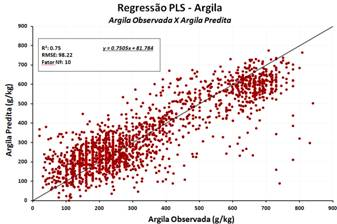
\includegraphics{figuras/image003}
\end{figure}

\section{Tipos de amostras}

Vários tipos de amostras foram recebidas durante o ano de 2014, a saber:

\begin{itemize}
  \item Amostras simples;
  \item Amostras em profundidade coletada com trado;
  \item Amostras de horizontes de perfis completos.
\end{itemize}

O recebimento de amostras variadas foi efetuado nesta etapa para avaliarmos as dificuldades na implementação do projeto.

\section{Métodos}

As amostras recebidas são catalogadas e uma alíquota é armazenada, recebendo uma sigla e a identificação do responsável pela amostra. Todos os procedimentos analíticos são realizados usando o sensor Fieldspec. Os dados espectrais são identificados com a mesma sigla da amostra, armazenados no banco de dados, e em seguida ligados ao arquivo MS Office Excel contendo os dados analíticos.

\section{Visitas}

Temos recebido pessoas de fora para visitar o laboratório ou mesmo acompanhar as leituras da própria amostra.

\section{Divulgação na Internet}

As atividades são divulgadas no site da \BESB{} e do Grupo de Pesquisa em Geotecnologia em Ciência do Solo (\GeoCIS) da ESALQ que dá apoio às atividades da BESB.

\begin{figure*}[tb!]
\begin{minipage}[t]{1\linewidth}
   \centering
   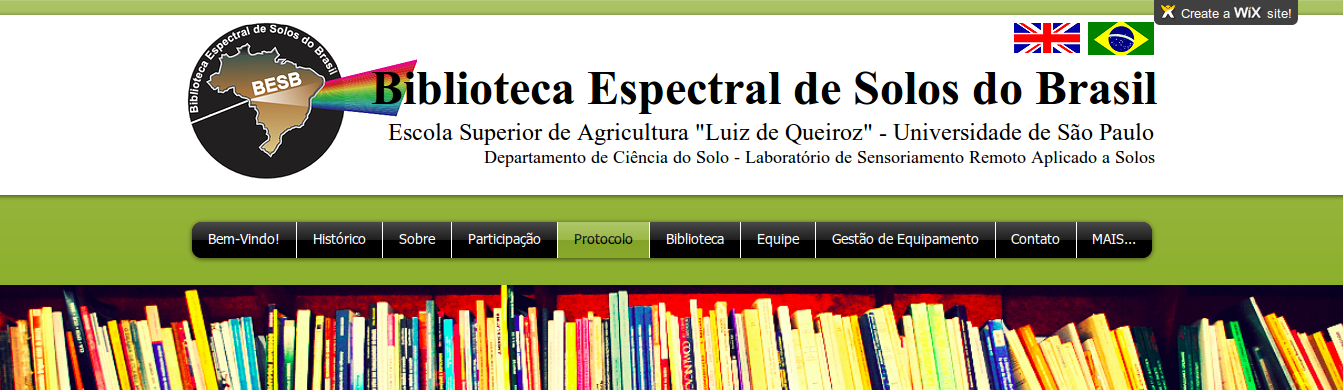
\includegraphics{figuras/image008}
   \caption{Banner da Biblioteca Espectral de Solos do Brasil.}
   \label{fig:banner}
\end{minipage}
\end{figure*}

\begin{figure}
  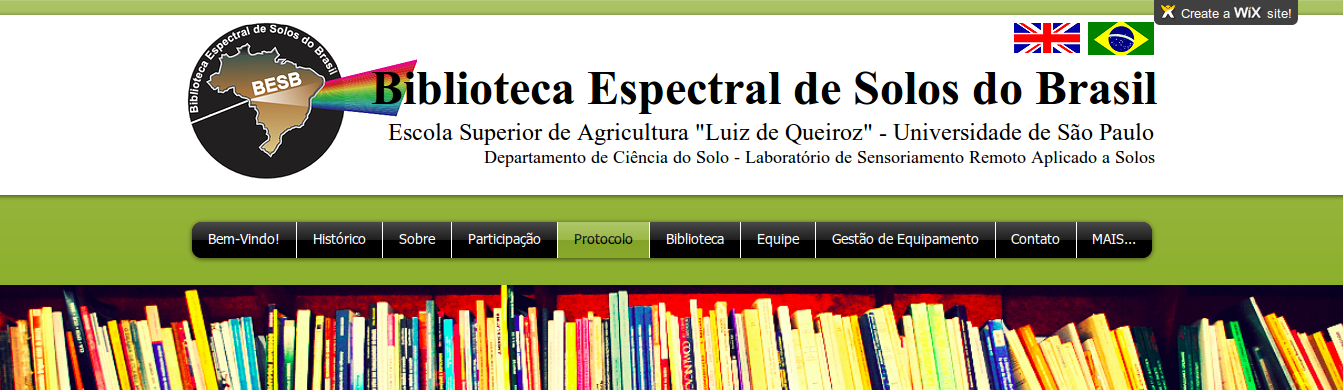
\includegraphics{figuras/image008}
\end{figure}

\section{Divulgação geral}

As BESB já foi divulgada em diversas oportunidades. São elas:

\begin{itemize}
  \item Reunião da FAO em Roma, Itália, em dezembro de 2013;
  \item Davis, Califórnia, EUA, em janeiro de 2014;
  \item College Station, Texas, EUA, em fevereiro de 2014;
  \item Simpósio de Iniciação Cientifica da USP, em dezembro de 2014;
  \item Programa Band Rural, em 2014;
  \item Revista FAPESP;
  \item E aqui na \pedometria.
\end{itemize}

\section{Grupo de pesquisa}

Foi criado o Grupo de Espectroscopia de Solos do Brasil (\GESB). O grupo se encontra em fase de análise no CNPq.

\section{Publicação}

A primeira publicação somente virá após o término do mestrado do aluno que esta fazendo o trabalho. Isto se dará em maio de 2015. Vai tratar desta primeira versão. Logo em seguida segue um novo aluno para partir para a nova e última etapa a seguir descrita. Também será publicado um relatório no formato de Atlas de Solos do Brasil contendo fotos e espectros.

\section{Apresentação e publicação do material}

O material será apresentado no Congresso Brasileiro de Ciência do Solo (CBCS) a ser realizado em Natal em agosto 2015, após o qual será submetido a publicação um artigo de caráter geral. Nele TODOS os colaboradores serão incluídos como co-autores. Esta será o que chamo de primeira versão. pois haverá uma segunda versão hum ano depois, finalizando a etapa de publicações gerais.
Se tudo correr bem, haverá uma palestra sobre o trabalho no CBCS.

\section{Próximas etapas}

O RECEBIMENTO DE AMOSTRAS CONTINUA!!! Mas a partir de agora somente serão aceitas:

\begin{itemize}
  \item amostras de perfis completos, OU
  \item amostras de tradagens completas em profundidade
\end{itemize}

As amostras DEVEM vir acompanhadas de foto do perfil e dados analíticos mínimos:

\begin{itemize}
  \item Granulometria;
  \item Química tradicional;
  \item Classificação taxonômica até o máximo nível categórico possível.
\end{itemize}

O georreferenciamento, apesar de desejado, não é obrigatório, sendo suficiente indicar apenas o município mais próximo. O protocolo para a coleta de perfis completos e uma planilha modelo para envio dos dados estão disponíveis no site da BESB (\href{http://bibliotecaespectral.wix.com/esalq#!protocolo/c1sc5}{acesse aqui}). 

\section{Forma de apresentação}

A \autoref{fig:curvas} mostra o que desejamos atingir na próxima etapa de desenvolvimento da BESB. Na primeira etapa 1, que ora finaliza, conseguimos avançar em direção a este objetivo. Mas a segunda etapa será mais restritiva, exigindo mais as análises e descrição do local e do perfil.

\begin{figure*}[tb!]
\begin{minipage}[t]{1\linewidth}
   \centering
   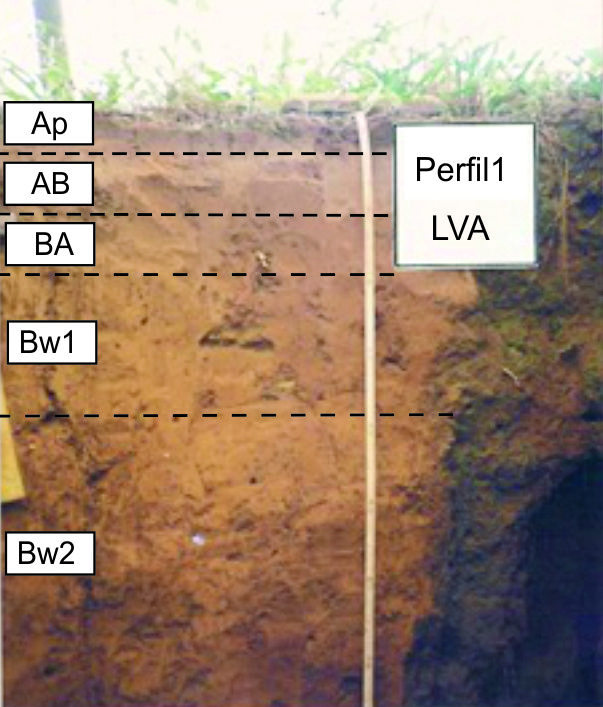
\includegraphics[width=0.49\textwidth]{figuras/lva.jpg}
   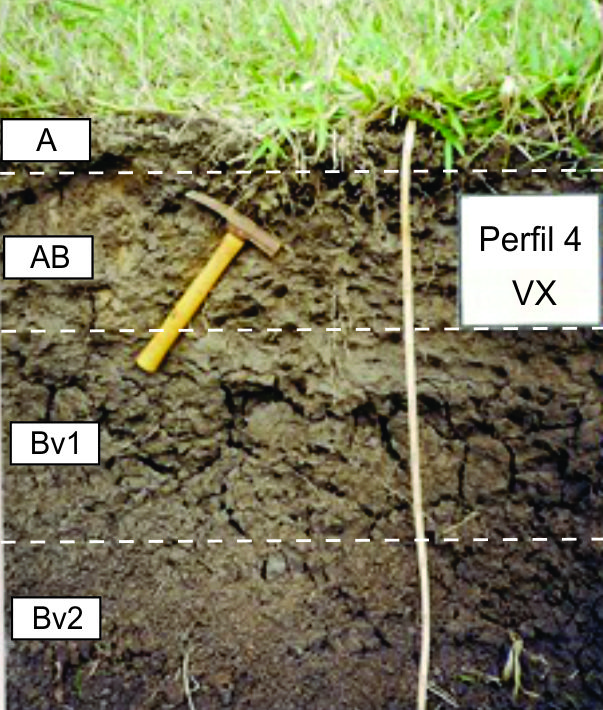
\includegraphics[width=0.49\textwidth]{figuras/vertissolo.jpg}
   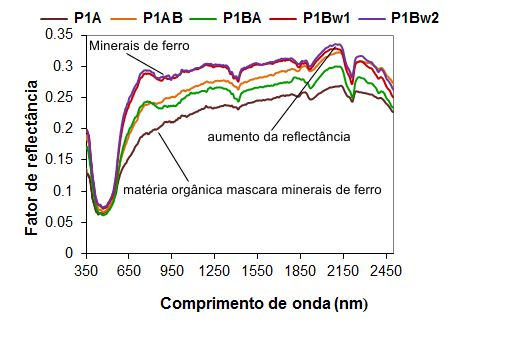
\includegraphics[width=0.49\textwidth, trim=0.5cm 0cm 1.5cm 0cm, clip]{figuras/curvas-lva.jpg}
   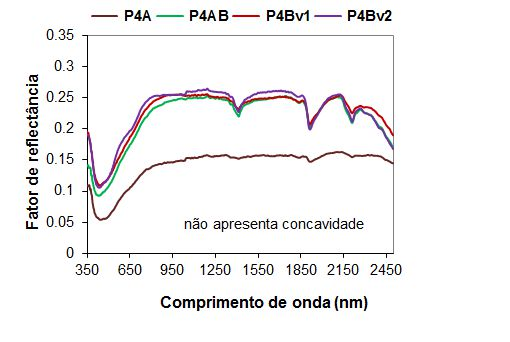
\includegraphics[width=0.49\textwidth, trim=0.5cm 0cm 1.5cm 0cm, clip]{figuras/curvas-vertissolo.jpg}
   \caption{Curvas espectrais dos horizontes de perfis estudados. Solo 1 -- Latossolo Vermelho-Amarelo com horizontes Ap, AB, BA, Bw1, Bw2. Solo 2 -- Vertissolo Háplico com horizontes A, E, Bv1 e Bv2.}
   \label{fig:curvas}
\end{minipage}
\end{figure*}

\section{Dúvidas frequentes}

A maior dúvida dos colaboradores é quanto aos direitos retidos sobre os dados. Muitos parecem ter dificuldade em compartilhar dados devido ao receio de não receber qualquer crédito autoral.

Queremos deixar claro que os dados enviados são de propriedade daquele que os enviou. A equipe da BESB apenas obtém os dados espectrais, e sim, publicaremos um primeiro trabalho, para preservar o nosso trabalho inicial. MAS é um trabalho MACRO, não regional, logo, o ‘dono’ dos dados poderá publicar artigos com os seus dados em caráter regional.

Além disso, os dados ficarão guardados aqui na ESALQ (onde nem eu nem ninguém poderá utiliza-los) e será enviado aos respectivos donos. Este método, permitirá que todos no Brasil, indo no site, saibam QUEM tem dados, e com isso, possam se contatar mutuamente para fazer trabalhos em conjunto fortalecendo a comunidade e aumentando os índices de publicação. De nossa parte o ganho será a citação do trabalho base (Mas com todos co-autores), o global, a citação da BESB e um atlas.

ESTOU TENDO CERTA DIFICULDADE EM CONVENCER ALGUNS COLEGAS. PRECISAMOS DE PERFIS COMPLETOS A PARTIR DE AGORA COM FOTOS. ISSO VAI GERAR UM ATLAS DE IMPACTO IMPORTANTE E FICAR POR GERAÇÕES. PECO A TODOS OS  QUE VEREM ESTE MAIL, REPASSEM A COLEGAS PEDÓLOGOS, SENSIBILIZANDO-OS AO CUSTO/BENEFICIO DESTA INICIATIVA. A PARTICIPAÇÃO DEVE SER DE PEDÓLOGOS QUE TEM ACERVOS OU AMOSTAS DE PERFIS COMPLETOS COM FOTOS E DESCRIÇÕES.

Vejam, o pedólogo não vai perder estes dados NEM que ele mesmo pense em  gerar artigos em espectroscopia, pois o que vira para nos será usado para um atlas e para uma publicação de caráter geral. Estas duas publicações NÃO inviabilizam publicações regionais, aprofundadas com os dados. Ademais, tem pedólogos que estão guardando material que nem sabem se um dia irão usar para espectroscopia! Com isso, o BRASIL vai ficar sem estes dados a disposição da comunidade. Mostrar um espectro num atlas não inviabiliza a publicação do processamento e estudo do mesmo! Ademais, no ATLAS, os nomes dos doadores estarão sendo divulgados!
 
Esta iniciativa é para deixar algo para o futuro do pais, para os novos pedólogos e gerações.
 
Continuo a disposição para esclarecimentos.
O projeto continua!
Abcs


19-34172109
 
QUEM ACREDITAR NA INICIATIVA, POR FAVOR REPASSEM AO MAIOR NUMERO DE COLEGAS PDOLOGOS POSSIVEL!!!! E QUE ENTREM EM CONTATO COMIGO!

\address{Alexandre Demattê\\
  Departamento de Ciência do Solo, ESALQ/USP\\
  \url{http://www.solos.esalq.usp.br/docentes.htm}\\
  \email{jamdemat@usp.br}}

\address{Alessandro Samuel-Rosa\\
  ISRIC - World Soil Information\\
  \url{http://www.soil-scientist.net}\\
  \email{alessandro.rosa@wur.nl}}
%%% Local Variables: 
%%% mode: latex
%%% TeX-master: 5th-edition.tex
%%% End: 